\subsection{Comparison of the CET and DCT Estimators}
\label{subsec:agit-cetdct}

The two estimators were compared in the daemon itself, with the encoder at 256 PPR (DIP 0011, 1024 counts per revolution), real-time (FIFO) scheduling, a 10~ms loop, and no torque channel, so that the estimator is the only thing that changes between runs. Five variants were run in turn: the DCT estimator with sampling windows of 5, 10, and 20~ms, and the two CET estimators of Section~\ref{subsec:agit-cet} (aligned and newest edge). Each variant ran three tests with the same schedules: an open-loop PWM staircase from 10 to 90~\% in steps of 10~\%, held 10~s each (test A), and closed-loop staircases of setpoints from 10 to 1500~rpm held 15~s each, once with the earlier gains $K_p = 1.5641$ and $K_i = 41.2249$ (test Bold) and once with the gains designed on the identified plant, $K_p = 0.2482$ and $K_i = 6.8691$ (test Bimc; Section~\ref{subsec:agit-pi-tuning}). The interior of every hold is analysed. The speed of every step is also computed from the index pulses (Section~\ref{subsec:agit-speed-test}) and is used as the reference for the bias. Each variant was run once, so a difference of 10 to 20~\% between two variants is inside the run-to-run scatter and is not claimed as a difference; the differences reported below as findings are factors of 3 to 11.

\paragraph{The DCT estimator.}
The earlier discrete-time (DCT) estimator was computed in the control loop. On every loop it read the position count and the system clock and formed the difference of each from the previous loop. It accumulated the count difference and the elapsed time until the elapsed time reached a configured window $T_w$, and then computed
\begin{equation}
    n = \left| \frac{\Delta c}{N} \right| \cdot \frac{60}{\Delta t}
    \label{eq:dct}
\end{equation}
with $\Delta c$ the accumulated count and $\Delta t$ the accumulated clock time. The value was held until the next window completed. This is the frequency-based method of Equation~2 in \citet{anuchin2019}, with the time taken from the loop clock. Three properties distinguish it from the CET estimator of Section~\ref{subsec:agit-cet}.
\begin{enumerate}
    \item The count increment is any integer and not a multiple of four, so each window carries one count of quantization, a speed step of $60/(T_w N)$, which is 11.7, 5.9, and 2.9~rpm for 5, 10, and 20~ms, and the duty-cycle and phase errors of the encoder are not cancelled.
    \item The elapsed time is the difference of two readings of the loop's own clock and not the time stamps of the edges. The count is read slightly before the clock, so a delay between the two readings enters the speed as a relative error equal to the delay divided by the window: 100~$\mu$s is 2~\% of a 5~ms window and 0.5~\% of a 20~ms window.
    \item The window is a threshold on the accumulated time, so the interval between refreshes is a whole number of loop periods and depends on the exact period of each loop. A window equal to a whole number of nominal periods is reached or missed depending on whether the periods are a little below or above nominal, and the refresh then waits for the next loop.
\end{enumerate}

\paragraph{Open loop.}
Table~\ref{tab:ol-sd} and Figure~\ref{fig:est-sd}a give the standard deviation of the raw speed in the open-loop staircase. The aligned CET estimator has 2.7 to 4.9~rpm from 230 to 2140~rpm, nearly constant over the range, and the newest-edge estimator is within 0.5~rpm of it at every step. The M/T error of Equation~\ref{eq:mt} is 0.1 to 0.5~rpm over this range (Table~\ref{tab:esterr}), so most of the CET scatter is the shaft-synchronous ripple of Section~\ref{subsec:agit-fft}. The DCT scatter grows with the speed, in proportion to it: from 7 to 8~rpm at 230~rpm to 51, 50, and 32~rpm at 2140~rpm for the windows of 5, 10, and 20~ms. That is 2.4, 2.3, and 1.5~\% of the speed, an equivalent timing uncertainty of 0.12, 0.23, and 0.30~ms for the window in question. This is the order of magnitude of the clock-reading delay of item~2 above and not of the count quantization of item~1, which does not depend on the speed. At 1300~rpm the DCT scatter is 31, 31, and 19~rpm against 3.6~rpm for aligned CET, a factor of 8.6, 8.6, and 5.3. Averaged over the steps from 30 to 80~\% PWM (770 to 2140~rpm) it is 34.5, 33.7, and 21.1~rpm for DCT at 5, 10, and 20~ms against 3.8~rpm for each CET estimator. The 20~ms window is the quietest DCT variant because it has the smallest count quantum and averages over the longest time, at the price of the longest delay.

\begin{table}[htbp]
    \centering
    \caption[Open-loop speed scatter by estimator]{Standard deviation of the raw speed (rpm) in the open-loop PWM staircase at 256 PPR, 10~s per step, one run per estimator. The 90~\% step is not usable for DCT: the 5 and 10~ms runs reached the 12\,000~rpm safety limit during that step (the 5~ms run before its interior could be analysed), and the 20~ms run contains a loop stall of 1.8~s.}
    \label{tab:ol-sd}
    \small
    \resizebox{\textwidth}{!}{\begin{tabular}{@{}rrrrrrr@{}}
\toprule
PWM % & speed rpm & DCT 5 ms & DCT 10 ms & DCT 20 ms & CET aligned & CET newest \\
\midrule
10.00 & 230.23 & 7.17 & 7.55 & 7.87 & 4.84 & 5.30 \\
20.00 & 502.40 & 11.81 & 13.06 & 7.36 & 3.28 & 3.22 \\
30.00 & 773.92 & 17.37 & 20.22 & 11.45 & 2.68 & 3.04 \\
40.00 & 1043.97 & 24.75 & 23.97 & 13.85 & 3.51 & 3.46 \\
50.00 & 1316.88 & 30.69 & 30.94 & 18.93 & 3.58 & 3.70 \\
60.00 & 1588.91 & 37.92 & 32.24 & 23.38 & 3.69 & 3.83 \\
70.00 & 1862.18 & 45.30 & 44.77 & 27.02 & 4.27 & 4.50 \\
80.00 & 2138.42 & 51.14 & 50.03 & 31.65 & 4.86 & 4.38 \\
90.00 & 2390.57 & -- & 1819.88 & 505.04 & 6.53 & 3.72 \\
\bottomrule
\end{tabular}
}
\end{table}

\begin{figure}[htbp]
    \centering
    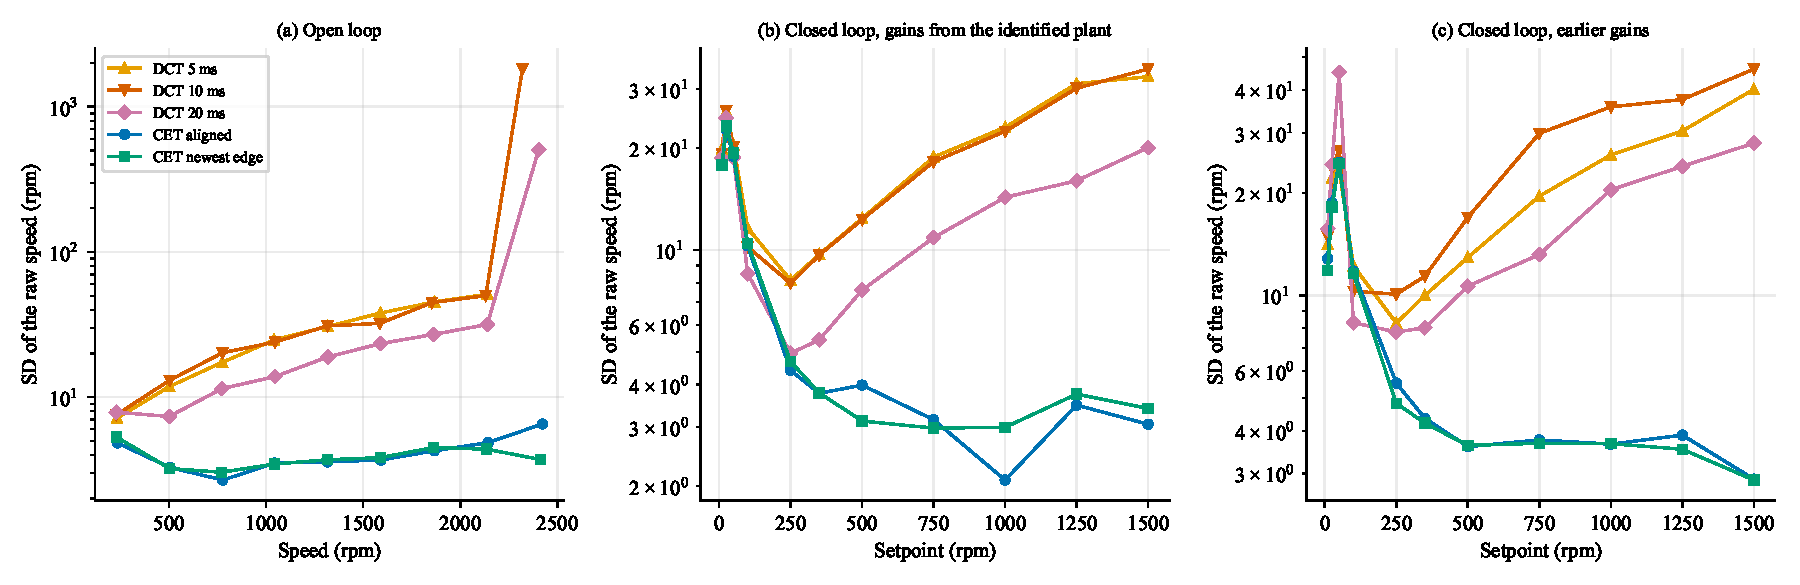
\includegraphics[width=\textwidth]{figures/fig_est_sd}
    \caption[Speed scatter against speed for five estimators]{Standard deviation of the raw speed for the three DCT windows and the two CET estimators at 256 PPR. (a) Open-loop staircase against speed. (b) Closed loop with the gains from the identified plant, against setpoint. (c) Closed loop with the earlier gains. One run per estimator.}
    \label{fig:est-sd}
\end{figure}

\paragraph{Spikes.}
The DCT estimator also produces isolated estimates far from the true speed. Counting the raw samples that differ from the local median by more than 50~\% at speeds above 100~rpm gives 851, 4524, and 1795 per million samples for DCT at 5, 10, and 20~ms, and 524 and 518 per million for the aligned and newest-edge CET estimators; the largest sample is 8.8 times the median for DCT at 10~ms and 3.6 times for CET. The same kind of sample ended two open-loop runs, DCT at 5 and 10~ms, at the 12\,000~rpm limit during the 90~\% step, where the shaft turns at about 2400~rpm. The CET figure is not zero, about one sample in two thousand, so no estimator is free of outliers, but DCT at 10~ms produces nine times as many as CET and DCT at 20~ms about three times as many. A lost edge was counted in three of the five variants (\texttt{quad\_err} equal to one for DCT at 5 and 10~ms and for newest-edge CET), so the spikes are not caused by lost counts. One plausible cause, which these logs do not test, is that the count read by the DCT estimator is updated when the callbacks are delivered and not when the edges occur, so a delayed delivery is followed by a burst that the estimator divides by a clock interval that did not stretch with it.

\paragraph{Accuracy against the index pulses.}
Scatter is not accuracy. Table~\ref{tab:est-acc} gives the mean of each estimator over each step, minus the speed from the index pulses, for speeds above 100~rpm. Every estimator is unbiased to within 0.1~\% except in the steps in which it spiked. The mean absolute bias is 0.002 to 0.008~\% for the aligned CET estimator, 0.002 to 0.018~\% for the newest-edge CET estimator, 0.007~\% for DCT at 5~ms, 0.03 to 0.06~\% for DCT at 20~ms, and 0.09 to 0.48~\% for DCT at 10~ms, where the last figure is dominated by a bias of $-3.8$~\% at the 90~\% step of test A. The DCT estimator at 10~ms is the only variant with a systematic bias, $-0.05$ to $-0.11$~\% in most steps; the cause is not identified. By Equation~\ref{eq:npo-unc} a speed bias of 0.1~\% is 0.2~\% in the Power number, small against the uncertainty of the torque (Section~\ref{subsec:agit-power}). The choice of estimator therefore changes the \emph{scatter} of the speed, and with it the behaviour of the control loop, much more than it changes the mean speed used in the $N_{Re}$--$N_{Po}$ curve.

\begin{table}[htbp]
    \centering
    \caption[Bias of each estimator against the index pulses]{Bias of the mean speed of each estimator against the speed from the index pulses, over the steps above 100~rpm. Tests: A, open loop; Bold, closed loop with the earlier gains; Bimc, closed loop with the gains from the identified plant. ``Steps'' is the number of steps analysed; the bias is in percent of the speed except the last column (rpm).}
    \label{tab:est-acc}
    \small
    \resizebox{\textwidth}{!}{\begin{tabular}{@{}rrrrrrr@{}}
\toprule
est & test & steps & mean bias pct & mean abs bias pct & max abs bias pct & mean bias rpm \\
\midrule
aligned & A & 9 & 0.006 & 0.008 & 0.050 & 0.129 \\
aligned & Bimc & 7 & 0.001 & 0.002 & 0.004 & 0.005 \\
aligned & Bold & 8 & 0.001 & 0.002 & 0.004 & 0.004 \\
dct10 & A & 9 & -0.481 & 0.481 & 3.805 & -10.868 \\
dct10 & Bimc & 8 & -0.065 & 0.095 & 0.233 & -0.466 \\
dct10 & Bold & 7 & -0.090 & 0.090 & 0.149 & -0.829 \\
dct20 & A & 9 & -0.055 & 0.056 & 0.261 & -0.882 \\
dct20 & Bimc & 8 & -0.010 & 0.040 & 0.154 & 0.024 \\
dct20 & Bold & 7 & -0.008 & 0.029 & 0.064 & -0.150 \\
dct5 & A & 8 & 0.007 & 0.007 & 0.019 & 0.074 \\
dct5 & Bimc & 7 & 0.007 & 0.007 & 0.011 & 0.050 \\
dct5 & Bold & 7 & 0.007 & 0.007 & 0.015 & 0.044 \\
newest & A & 9 & -0.001 & 0.002 & 0.006 & -0.017 \\
newest & Bimc & 8 & -0.012 & 0.018 & 0.109 & -0.004 \\
newest & Bold & 8 & -0.003 & 0.010 & 0.047 & 0.007 \\
\bottomrule
\end{tabular}
}
\end{table}

\paragraph{Age of the estimate.}
The firmware logs the age of the snapshot in use, the daemon clock minus the time stamp of the snapshot, with half of the round trip of the clock request (about 50~$\mu$s) subtracted. Table~\ref{tab:age} gives it against the maximum that the geometry of Section~\ref{subsec:agit-cet} predicts, $T_a$ for the aligned and $T_a/4$ for the newest-edge estimator. The newest-edge estimator has the smaller age at every speed: by 46~\% at 100~rpm (median 1.00 against 1.85~ms), 28~\% at 250~rpm, 15~\% at 500~rpm, and 1 to 4~\% at 1000 and 1500~rpm, where $T_a$ is below 0.25~ms and no longer fixes the age. The measured age exceeds the predicted maximum for the newest-edge estimator at every speed and for the aligned estimator from 250~rpm. At 1000 and 1500~rpm the median is 0.74 to 0.78~ms for both estimators, against predicted maxima of 0.04 to 0.23~ms. The excess is the same for both estimators, so it is a delay that does not come from the estimator: the transit of the edge through the pigpio notification stream to the daemon, which the time stamps do not contain. It is small against the 5~ms of $T_s/2$ in Equation~\ref{eq:delay}. The 95th percentile of the age at 500~rpm is 1.43~ms for the aligned and 1.13~ms for the newest-edge estimator. At 350~rpm the aligned run has one age of 10.9~ms, a loop that was served late, the same kind of event as the late wake-ups of the loop timing of Section~\ref{sec:plat-timing}.

\begin{table}[htbp]
    \centering
    \caption[Measured age of the speed estimate]{Age of the snapshot in use (microseconds) for the two CET estimators, from the log of the daemon. The prediction is the maximum of the geometric argument of Section~\ref{subsec:agit-cet}, and the aligned period is $T_a = 60\times10^{6}/(256\,n)$~$\mu$s. ``rtt'' is the round trip of the clock request.}
    \label{tab:age}
    \small
    \resizebox{\textwidth}{!}{\begin{tabular}{@{}rrrrrrrrr@{}}
\toprule
est & target & age med us & age p95 us & age max us & age raw med us & clock rtt us & Ta us & predicted max us \\
\midrule
aligned & 100.0 & 1849.2 & 3164.5 & 4012.6 & 1874.5 & 52.1 & 2343.8 & 2343.8 \\
aligned & 250.0 & 1138.4 & 1832.1 & 2556.0 & 1166.0 & 51.5 & 937.5 & 937.5 \\
aligned & 350.0 & 995.6 & 1639.1 & 10916.7 & 1025.5 & 51.3 & 669.6 & 669.6 \\
aligned & 500.0 & 905.1 & 1428.6 & 1634.1 & 931.5 & 50.3 & 468.8 & 468.8 \\
aligned & 1000.0 & 782.1 & 1258.5 & 1437.2 & 808.5 & 51.9 & 234.4 & 234.4 \\
aligned & 1500.0 & 750.4 & 1206.4 & 1781.9 & 779.0 & 51.8 & 156.2 & 156.2 \\
newest & 100.0 & 996.9 & 1479.7 & 1850.2 & 1023.0 & 46.9 & 2343.8 & 585.9 \\
newest & 250.0 & 822.2 & 1204.6 & 1425.6 & 846.5 & 46.9 & 937.5 & 234.4 \\
newest & 350.0 & 798.8 & 1168.4 & 1360.6 & 823.5 & 45.7 & 669.6 & 167.4 \\
newest & 500.0 & 766.5 & 1131.3 & 1476.8 & 790.5 & 46.5 & 468.8 & 117.2 \\
newest & 1000.0 & 748.0 & 1098.2 & 1337.3 & 774.5 & 46.7 & 234.4 & 58.6 \\
newest & 1500.0 & 740.0 & 1088.9 & 1221.3 & 764.0 & 47.6 & 156.2 & 39.1 \\
\bottomrule
\end{tabular}
}
\end{table}

The delay was also estimated from the slope of the phase of the first harmonic of the ripple, folded against the shaft angle with the index pulses (Section~\ref{subsec:agit-fft}). The slope gives 15.7 and 14.8~ms for the two CET estimators and 29.4 and 27.0~ms for DCT at 10 and 20~ms, but $-7$~ms for DCT at 5~ms, which is not possible, and it rests on three speeds, 230 to 780~rpm, where the line is at most 2.5~rpm. It is not used here; the age of Table~\ref{tab:age} is the measurement of the delay.

\paragraph{Closed loop.}
With the PI controller closed on the estimate (Table~\ref{tab:cl-sd}, Figure~\ref{fig:est-sd}b and~c), the estimators are indistinguishable at 100~rpm and below and differ a great deal above. At setpoints from 10 to 100~rpm every estimator has a standard deviation of 8 to 27~rpm with either set of gains, except DCT at 20~ms at 50~rpm with the earlier gains (45~rpm), so that scatter belongs to the motor and its drive at low speed and not to the estimator; Section~\ref{subsec:agit-pi-tuning} treats that range. From 250~rpm the CET estimators hold the speed within 2 to 5.5~rpm at every setpoint with either set of gains, while the scatter of DCT grows with the setpoint: with the gains of the identified plant it is 8 to 33~rpm for DCT at 5~ms, 8 to 34~rpm at 10~ms, and 5 to 20~rpm at 20~ms. At 1500~rpm the DCT scatter is 32.6, 34.3, and 20.1~rpm against 3.05~rpm for aligned CET, which is 10.7, 11.2, and 6.6 times larger. Averaged over the setpoints from 250 to 1500~rpm the ratio is 5.7, 5.6, and 3.3. With the earlier, higher gains the DCT scatter at 1500~rpm is 40, 46, and 28~rpm, a ratio of 14, 16, and 9.7, so the lower gains reduce the DCT scatter by 20 to 28~\% but do not remove it, and leave the CET scatter unchanged. That the CET scatter does not depend on the gains and the DCT scatter does only in part points to the DCT estimate itself, with its spikes and its irregular refresh, and not to the tuning. These logs do not separate the contribution of the delay from that of the noise of the estimate, but the DCT window of 5~ms, which refreshes on every loop and adds the least delay of the three, is not quieter than the 20~ms window, which indicates that the noise of the estimate and not its delay dominates the scatter in this test.

\begin{table}[htbp]
    \centering
    \caption[Closed-loop speed scatter by estimator, identified-plant gains]{Standard deviation of the raw speed (rpm) in the closed-loop staircase at 256 PPR with the gains from the identified plant, $K_p = 0.2482$ and $K_i = 6.8691$, 15~s per setpoint, one run per estimator. The results for the earlier gains, $K_p = 1.5641$ and $K_i = 41.2249$, are in Figure~\ref{fig:est-sd}c.}
    \label{tab:cl-sd}
    \small
    \begin{tabular}{@{}rrrrrr@{}}
\toprule
setpoint rpm & DCT 5 ms & DCT 10 ms & DCT 20 ms & CET aligned & CET newest \\
\midrule
10.00 & 19.88 & 19.25 & 18.67 & 17.82 & 17.85 \\
25.00 & 25.66 & 25.78 & 24.59 & 22.71 & 23.30 \\
50.00 & 20.44 & 20.20 & 18.76 & 18.94 & 19.35 \\
100.00 & 11.61 & 10.21 & 8.51 & 10.29 & 10.47 \\
250.00 & 8.13 & 7.97 & 4.95 & 4.40 & 4.68 \\
350.00 & 9.70 & 9.66 & 5.42 & 3.77 & 3.78 \\
500.00 & 12.40 & 12.30 & 7.61 & 3.98 & 3.12 \\
750.00 & 18.83 & 18.24 & 10.88 & 3.15 & 2.97 \\
1000.00 & 23.07 & 22.45 & 14.32 & 2.09 & 2.99 \\
1250.00 & 31.04 & 30.11 & 16.03 & 3.48 & 3.75 \\
1500.00 & 32.57 & 34.31 & 20.10 & 3.05 & 3.40 \\
\bottomrule
\end{tabular}

\end{table}

\paragraph{Which estimator is used.}
The aligned CET estimator is selected. From 250~rpm upward its scatter is the smallest or within a few tenths of a rpm of the smallest in every test, it has the smallest bias against the index pulses, no lost edge in any run, and a bounded delay. The newest-edge estimator is equivalent in scatter and bias and has the smaller age, but the difference in age is a few tenths of a millisecond at the speeds of the experiment (above 250~rpm) and each variant was run once, so the logs do not distinguish the two. All measurements of the following sections use the aligned estimator with the loop period of 10~ms, and the DCT estimator is not used for any measurement of the $N_{Re}$--$N_{Po}$ curve. The conclusion that CET is better than DCT at the same encoder setting, loop, and gains rests on factors of 3 to 11 in closed loop and of 5 to 9 in open loop above 1000~rpm, far larger than the run-to-run scatter, and it holds for every DCT window tried.

\paragraph{Earlier logs.}
Two earlier sets of logs are superseded by the comparison above. The 256 PPR sweeps logged by the dashboard on 2~September (DCT) and on 4 and 7~September (CET) gave a mean standard deviation of 40 to 56~rpm with DCT and 4.9 to 8.6~rpm with CET, the same order as Table~\ref{tab:ol-sd}, but they were taken on different days and under different conditions. The harness sweeps of the earlier estimator, 1 to 3~rpm for DCT, disagree with the 8 to 54~rpm of the daemon, and a harness closed-loop staircase with DCT at 20~ms refreshed the estimate on only 39~\% of the loops; the new runs, made in the same daemon with the same encoder setting, replace them.

